\chapter{Optimization}

\section{Optimization in data analysis}
Lots of problem in statistical learning can be formulated as \textit{optimization problems} where we have to \textit{minimize} or \textit{maximize} an \textbf{objective function}. % NON HA MOLTO SENSO QUESTO PERODO: Thus, optimization is important because we need to know how solve the optimization problems in a computationally efficient way.
Since some optimization problems often cannot be solved in closed form there are some specific algortihm called \textbf{optimization algorithms}.

Many statistical learning tasks can be traced back to the following formulation:
\[
    \min_\beta J(\beta)
\]

where $J$ is the \textit{objective function}. Specifically, we call it \textit{cost function} if the problem is a \textit{minimization} problem, and \textit{reward function} if the problem is a \textit{maximization} problem.

This type of problem is also referred to as \textit{unconstrained} minimization problem. In an unconstrained problem, the parameter $\beta$ has no constraints on the value it can take within its definition space ($\R^p$).
There are, however, constrained problems where $\beta$ could take on a physical meaning: probability vector, temperature value. And consequently it takes on physical constraints.
In that cases, we need to use algorithms that are able to handle the constraints. We will see unconstrained problems.

\subsection{Objective Function}

Assume that we have \textbf{random data} $D \in \mathcal{D}$ as feature-label pairs: $D = (X,Y)$.

\begin{definition}
    The \textbf{loss} function $Q_\beta(d)$ is a function of $d \in D$ parameterized by $\beta \in \mathbb{R}^p$.
\end{definition}

The loss function tells, for a choice of $\beta$, how much we are losing for a specific feature-label pair $d$.

\begin{definition}
    The \textbf{cost} function, also known as \textit{risk} or \textit{objective} function, is defined as the loss function averaged over $D$:
    \[
        J(\beta) = \E{}{Q_\beta(D)}
    \]
\end{definition}

Our goal is to find the $\beta$ that minimizes the cost function.

%Another thing is the more we relax the assumptions, the less information we get. \textit{The less we ask, the less we get.} For example, when I work under the assumption that

%A \textbf{performance guarantee} means that whatever we do the dataset seems to work, meaning that we can apparently obtain some information.

\begin{definition}
    We can define statistical learning as an optimization problem as the \textit{unconstrained minimization} of the \textit{cost function}:
    \[
        \min_{\beta \in \mathbb{R}^p} J(\beta) = \E{}{Q_\beta(D)}
    \]
\end{definition}

For example in the regression case we minimize the mean-square-error while in the classification case we minimize the conditional cross-entropy.

\paragraph*{Linear Regression}
In the regression case, in particular linear regression, the loss function is the error:
\[
    Q_\beta(d) = Q_\beta(x,y) = (x^T\beta - y)^2
\]
Then the cost function will be the well known mean square error:
\[
    J(\beta) = \E{}{(X^T \beta - Y)^2}
\]

\paragraph*{Logistic Regression}
In the classification case, logistic regression particularly, the loss function is the cross-entropy:
\[
    Q_\beta(d) = Q_\beta(x,y) = \log\left(1+e^{-y x^T \beta}\right)
\]
Then the cost function will be the \textit{conditional} cross-entropy:
\[
    J(\beta) = \E{}{\log\left(1+e^{-y x^T \beta}\right)}
\]

Note that this is the very same function seen in the previous chapter:
\[
    J(\beta) = \E{}{\log\left(\frac1{\hat\mu_\beta(y \mid x)}\right)} = \E{}{\log\left(\frac 1{1+e^{-y f(x)}}\right)} =  \E{}{\log\left(1+e^{-y f(x)}\right)}
\]
\section{Problem assumptions}
\begin{remark}
    Given the cost function $J: \beta \in \mathbb{R}^{p} \to  j \in \mathbb{R}$, $\nabla J(\beta)$ is the gradient of the cost function and it is a vector of dimensions $p \times 1$, where each element is $\frac{\partial J(\beta)}{\partial \beta_i}$. The norm we are going to use is the \textbf{euclidean norm}.
\end{remark}

\subsection{Lipschitz Continuity}
Let's informally recall the definition of continuity. If two points $x_1$ and $x_2$ become closer since the difference $x_1 - x_2 \to 0$, then the values of the function evaluated in those two points also becomes closer, that is the difference between the two points becomes closer to zero.
More formally:
\begin{definition}
    A function $f(x)$ is \textbf{continuous} at a point $x_0$ if:
    \[
        \forall \epsilon > 0\exists \delta=\delta(\epsilon) > 0\;|\;|x-x_0| < delta\implies |f(x)-f(x_0)| < \epsilon\\
        x,x_0\in Dom(f)
    \]
\end{definition}

When we say a function is continuous, we don't know that is the rate with which they become closer. This is why we need to introduce the \textbf{Lipschitz-continuity} of the gradient.

\begin{definition}
    A function is defined \textbf{Lipschitz continuous} if:
    \[
        \forall \beta_1, \beta_2 \colon \| \nabla J(\beta_2) - \nabla J(\beta_1)\| \leq \delta \|\beta_2 - \beta_1\|
    \]
    i.e. the difference of the gradient compute for the parameters $\beta_1, \beta_2$ is upper bounded by the difference of the parameters times a constant $\delta > 0$, called \textbf{Lipschitz constant}.
\end{definition}

When the gradient is Lipschitz-continuous we usually say \textit{the gradient varies smoothly}.

This condition is even stronger than continuity because in addition to affirming the previous condition it also indicates the rate at which the two values of the function approach each other.
Therefore, the value that the norm of the difference between the two functions assumes is limited above by the norm of the difference between the two points multiplied by a certain constant.
The larger this constant is, the more margin of variation we are giving to the function.

\begin{theorem}
    \[
        \text{Lipschitz continuity} \implies \text{continuity}
    \]
\end{theorem}
\subsection{Convexity}
Let's introduce the definition of \textbf{convex combination}.
\begin{definition}
    A \textbf{convex combination} is a sum of two quantites weighted respectively by the coefficient $p$ and $1-p$.
    \[
        c = p x_1 + (1-p) x_2
    \]
    By definition, the convex combination of $x_1$ and $x_2$ always lies in between of $x_1$ and $x_2$.
\end{definition}

There are more levels of convexity, we are going to introduce the \textit{convex} function, the \textit{strictly convex} function and the \textit{strongly convex} function.
\subsubsection*{Simple Convexity}

\begin{definition}
    A function $f(x)$ is \textbf{convex} if for every $x_1, x_2$, $x_1 \neq x_2$ and for every $p \in (0,1)$, the function evaluated in the convex combination of $x_1$ and $x_2$ lies always below the chord that is described by the convex combination.
    \[
        f(p x_1 + (1-p) x_2) \leq p f(x_1) + (1-p) f(x_2) \qquad \forall \alpha \in (0,1) \text{ and } \forall x_1 \neq x_2
    \]
\end{definition}

So, in the context of optimization problems in statistical learning, another assumption made is that the cost function $J(\beta)$ need to be \textit{convex}:
\[
    J(\alpha \beta_1 + (1-\alpha)\beta_2) \leq \alpha J(\beta_1) + (1-\alpha)J(\beta_2) \qquad  \forall \alpha \in (0,1) \text{ and } \forall \beta_1 \neq \beta_2
\]

\begin{figure}[H]
    \centering
    \begin{tikzpicture}[scale=2]
        % Axis
        \draw[thick, ->] (-0.5,0) -- (4,0) node[anchor=north west] {$\beta$};
        \draw[thick, ->] (0,-0.5) -- (0,3) node[anchor=south east] {$J(\beta)$};
        % Parabola  
        \draw[scale=1,domain=1:3,smooth,variable=\x,blue] plot ({\x},{2*(\x-2)^2 + 0.5});
        % Lines
        \draw[dashed] (1.5,0) -- (1.5,1);
        \draw[dashed] (0,1) -- (1.5,1);
        \filldraw[black] (1.5,1) circle (1pt);

        \draw[dashed] (2.7,0) -- (2.7,1.48);
        \draw[dashed] (0, 1.48) -- (2.7,1.48);
        \filldraw[black] (2.7,1.48) circle (1pt);

        \draw[dashed] (2,0) -- (2,1.2);
        \draw[dashed] (0,0.5) -- (2,0.5);

        \filldraw[black] (2,0.5) circle (1pt);
        \node at (2,1.2) {$\times$};

        \draw[red] (1.5,1) -- (2.7,1.48);
        % Labels
        \node[below] at (1.5,0) {$\beta_1$};
        \node[below] at (2.7,0) {$\beta_2$};
        \node[below] at (2,0) {$\beta_\alpha$};

        \node[left] at (0,1) {$J(\beta_1)$};
        \node[left] at (0,1.48) {$J(\beta_2)$};
        \node[left] at (0,0.5) {$J(\beta_\alpha)$};

    \end{tikzpicture}
    \caption{Convex function}

\end{figure}
The most frequent convention in optimization is doing \textbf{minimization}, and thus assuming that the cost function is convex. However, if we need to solve a \textit{maximization problem}, then we would need a \textit{concave} function.
However, is not critical to have a convex function, because we can always minimize the negative of the function.
\callout{Note}{Some books indicate the convexity with $\text{convex}-\cup$ and the concavity with $\text{convex}-\cap$.}

\begin{definition}
    A function $J(\beta)$ is said to be \textbf{strictly convex} if:
    \[
        J(\alpha \beta_1 + (1-\alpha)\beta_2) < \alpha J(\beta_1) + (1-\alpha)J(\beta_2) \qquad \forall \alpha \in (0,1) \text{ and } \forall \beta_1 \neq \beta_2
    \]
\end{definition}

The unique difference from the convexity is that the inequality is strict.

\begin{definition}
    A function $J(\beta)$ is said to  be \textbf{strongly convex} if:
    \[
        J(\alpha \beta_1 + (1-\alpha)\beta_2) \leq \alpha J(\beta_1) + (1-\alpha)J(\beta_2) - \frac{\nu}{2} \alpha (1-\alpha) \| \beta_1 - \beta_2 \|^2
    \]
    \[
        \forall \alpha \in (0,1) \text{ and } \forall \beta_1 \neq \beta_2
    \]
    where $\nu >0 $ is the \textbf{strong-convexity constant}.
\end{definition}

The strong convexity is again a stronger condition about the convexity.

\begin{theorem}
    For the convexity, we have the following implications chain:
    \[
        \text{strong convexity} \implies \text{strict convexity} \implies \text{convexity}
    \]
\end{theorem}
Since the term $\frac{\nu}{2} \alpha (1-\alpha) \| \beta_1 - \beta_2 \|^2$ is always positive, where $\nu>0$ is the \textbf{strong convexity constant}, then we have that even if the function will be equal to the right member, it will be always under the chord, thus implying the strict convexity.

\subsubsection*{Convexity when the function is twice differentiable}
\paragraph*{Hessian matrix}
The Hessian matrix, indicated with $\nabla^2 J(\beta)$, is the matrix of second derivatives of a function. It is a matrix of dimensions $p \times p$, where each element $(i,j)$ is $\frac{\partial^2 J(\beta)}{\partial \beta_i \partial \beta_j}$.
The Hessian matrix is a \textbf{real} matrix since the function $J$ is real, and is a \textbf{simmetric} matrix.

\begin{theorem}
    A \textbf{real} and \textbf{symmetric} matrix is \textbf{diagonalizable} and has \textbf{real eigenvalues}.
\end{theorem}

It is useful to introduce the following definitions about the comparison of matrices.

\begin{definition}
    A matrix is said to be \textbf{positive definite} if all of its eigenvalues are positive. The notation $A > B$ for two symmetric matrices $A$ and $B$ means that $A-B$ is a \textbf{positive definite matrix}.
\end{definition}

\begin{definition}
    A matrix is said to be \textbf{positive semi-definite} if all of its eigenvalues are non-negative. The notation $A \geq B$ for two symmetric matrices $A$ and $B$ means that $A-B$ is a \textbf{positive semi-definite matrix}.
\end{definition}
For the previous defintions we can also use the symbol $\succ$ and $\succeq$.

Hovewer, given two matrices real and symmetric $A$ and $B$, the eigenvalues of $A-B$ aren't equal to the difference of the eigenvalues of $A$ and $B$. This is true if and only if states that $AB=BA$ (commutative property). The motivation behind this must be found into the theory of the \textbf{spectral decomposition} of a matrix.

We can rewrite the definitions of convexity in terms of the Hessian matrix.
\begin{definition}
    A function $J(\beta)$ is said to be \textbf{convex} if:
    \[
        \nabla^2 J(\beta) \geq 0 \ \forall \beta
    \]
\end{definition}

For example, let us consider the one dimensional case: if the second derivative is positive, then the function is convex.

\begin{definition}
    A function $J(\beta)$ is said to be \textbf{strictly convex} if:
    \[
        \nabla^2 J(\beta) > 0 \ \forall \beta
    \]
\end{definition}

\begin{definition}
    A function $J(\beta)$ is said to be \textbf{strongly convex} if:
    \[
        \nabla^2 J(\beta) \geq \nu I \ \forall \beta
    \]
    where $\nu > 0$ is the \textbf{strong-convexity constant}.
\end{definition}

Since for the identity matrix the commutative property holds, then the strong convexity property can be also seen as asking that the eigenvalues of $\nabla^2 J(\beta)$ are greater or equal $\nu$ for each possible value of $\beta$ (and so for each possible diverse matrix) that represent the eigenvalues of the matrix $\nu I_p$.

The parabola is the most common example of a strongly convex function.

An example of function that is not strongly convex but convex is the exponential function $e^{-x}$, because we cannot find a $\nu$ such that the function is greater or equal than that threshold. This is also because the exponential function is bounded from below by zero.

\begin{theorem}
    The MSE cost used in linear regression is strongly convex if the covariance matrix $\E{}{X^TX}$ is invertible.
\end{theorem}

\begin{proof}
    First we are going to prove that the Hessian matrix of the MSE cost is $\nabla^2 J(\beta) = 2 \E{}{X^TX}$.

    Let $X \in \mathbb{R}^{1 \times p}$ be the matrix of the features, $\beta \in \mathbb{R}^{p \times 1}$ and $Y \in \mathbb{R}$ be the target variable.
    Let us compute the gradient of the MSE cost:
    \begin{align*}
        \nabla J(\beta) = \nabla_\beta \E{}{(X \beta - Y)^2} =  \E{}{\nabla_\beta(X \beta - Y)^2} \\ = \E{}{\nabla_\beta(\beta^T X^T X \beta - 2 \beta^T X^T Y + Y^T Y)} = \\
        = \E{}{2 X^T X \beta - 2 X^T Y}
    \end{align*}
    Then we can compute the Hessian matrix:
    \begin{align*}
        \nabla^2 J(\beta) = \nabla_\beta \nabla_\beta J(\beta) = \nabla_\beta \E{}{2 X^T X \beta - 2 X^T Y} = \\
        = \E{}{2 X^T X} = 2 \E{}{X^T X}
    \end{align*}

    We know that if the predictors are centered to zero, $\E{}{X^TX}$ is an estimator of the variance covariance matrix and that matrix is a \textit{positive defined} and \textit{simmetric} matrix.

    If, by hypothesis, the covariance matrix is invertible, then its determinant is non-zero. Since the determinant of the covariance matrix is the product of its eigenvalues, then all of its eigenvalues are (also) non-zero.
    By consequence we have satisfied the conditions for the strict convexity:
    \[
        \text{det}\nabla^2 J(\beta) = \prod_{i=1}^{p} \lambda_i \neq 0 \implies \lambda_i > 0  \forall i \implies \text{Strict Convexity}
    \]

    A final observation is that the hessian matrix computed is \textbf{independent} from $\beta$. This means that the eigenvalues are the same for each value of $\beta$ and so there will be a value that minor all the eigenvalues that can be a candidate for the strong convexity constant $\nu$. Once defined $\nu$, we can say that the MSE cost is strongly convex.
    
    % Since the covariance matrix is positive semi-definite, then all of its eigenvalues are non-negative. Since the covariance matrix is then the determinant of the covariance matrix is non-zero, which means that all of its eigenvalues are non-zero. Thus, the eigenvalues of the covariance matrix are positive, and greater then the minimum eigenvalue $\lambda_{min} = \nu$, which proves the strong convexity of the MSE cost.
\end{proof}

\section{Gradient Descent}
Finding the minimum of a function is not an easy problem because we need to find the point where the derivative is zero; but this alone does not guarantee that we have found the minimum, because it could be a maximum or a saddle point. And even if we ascertain that the point is a point of minimum, we don't know if it is a local or global minimum.

So algorithms like \textbf{gradient descent} are very useful when our problem has a complex formulation.
The basic idea of the gradient descent is to start from a random point and then move in the opposite direction of the gradient, which is the direction of the steepest descent. The gradient descent is an iterative algorithm.

\begin{algorithm}[H]
    \SetAlgoLined
    Set a starting point $\beta_0$ \\
    \For{$i=1,2,\dots$}{
        $\beta_{i} = \beta_{i-1} - \mu \nabla J\beta_{i-1}$
    }
    \caption{Gradient Descent}
\end{algorithm}

\begin{figure}
    \centering
    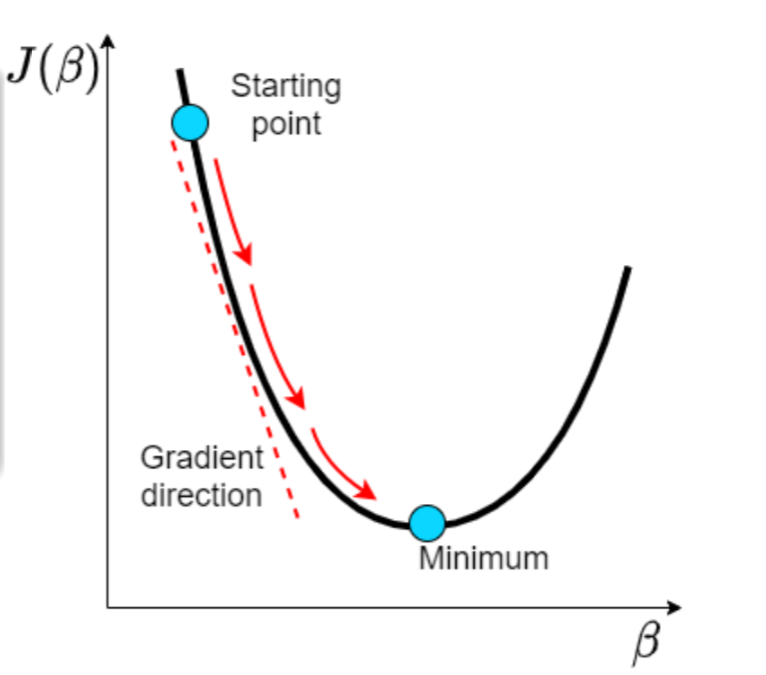
\includegraphics[width=0.5\textwidth]{./figures/chapter_6/graphicgradientdescent.png}
    \caption{Gradient Descent}
    \label{fig:gradient_descent}
\end{figure}

A graphical representation of the gradient descent is shown in Figure \ref{fig:gradient_descent}.

Each time we update the parameters in the gradient descent algorithm, we are moving by a step that is proportional to $\mu$, which is usually called \textit{step-size}. We can show that if $\mu$ is small enough (where small is determined by $\delta$ and $\nu$), then the gradient descent algorithm converges to the minimum of the function with a certain \textbf{convergence rate}. 
But if we choose a step-size that is too large, then the algorithm may not converge.

When the value of $J(\beta_i)$ is close to the minimum, the gradient could start to oscillate around the minimum, and the algorithm could not converge. To relax this problem we requested the \textit{Lipschitz continuity} of the gradient tha tells us that when $\beta_i$ is close to $\beta^\ast$, also the module of the gradient will reduce, in order to avoid the oscillation.
The strong convexity assumption, if satisfied, guarantees that the minimum is unique. 

\subsection{Convergence}
\subsubsection*{Constant step-size}
If we use a \textbf{constant step-size}, then we can show that for $\mu$ smaller than a certain value (which depends on the Lipschitz constant $\delta$ and the strong-convexity constant $\nu$), the gradient descent converges to the \textbf{exact minimizer}.
Viceversa, if the value of $\mu$ is too large, then the gradient could oscillate around the minimum and the algorithm may not converge.

The algorithm converges at a \textit{geometric} rate on the order $O(\rho^i)$ where $\rho \in (0,1)$ is a decreasing function of the step-size $\mu$ and also depends on $\delta$ and $\nu$.

\subsubsection*{Decaying step-size}
We can also choose to use a \textbf{decaying step-size}. 
If we consider an iteration-dependent step-size $\mu = \mu(i)$, with $\sum_{i=0}^{+\infty} \mu(i) = +\infty$ and $\lim_{i \to +\infty} \mu(i) = 0$ (we're asking that $\mu$ decreases but not too slowly), the gradient descent converges to the \textbf{exact minimizer} with a \textit{non-geometric} rate.
In practice, the convergence is still guaranteed but it is slower.

A typical choice is $\mu(i) = \frac{\tau}{i + 1}$ with $\tau > 0$, yielding a convergence rate of $O(\frac{1}{i^{2 \nu \tau}})$.

Since now, there aren't particular motivation to choose a decaying step-size because the convergence rate is slower and, even if we have the convergenze, we have to satisfy the previosly listed constraints on $\mu(i)$.

\subsection{Gradient Descent Limitations}

In practice, we cannot compute the cost function $\E{}{Q_\beta(D)}$ because we do not know the distribution of $D$. However, by using our dataset $\{d_i\}_{i=1}^n$, we can compute the empirical risk:
\[
    J_{emp}(\beta) = \frac{1}{n}\sum_{i=1}^{n} Q_\beta(d_i)
\]

In practice, we do not use this empirical risk because the computation of the gradient:
\begin{itemize}
    \item it is not suited to large datasets, since we need to compute the gradient for each iteration of the algorithm
    \item it is not suited in the case of online learning, since our dataset changes over time and we want to track the evolution of the data
    \item it is not suited for distributed application
\end{itemize}

\section{Stochastic Gradient Descent}
The solution to the limitations of the gradient descent is using an \textbf{instantaneous approximation of the gradient} based on individual samples:
\[
    \hat{\nabla J_i}(\beta) = \nabla Q_\beta(d_i)
\]
We are moving from the expectation of the loss function to the empirical risk by applying the law of large numbers and then we use an approximation of the gradient of this empirical risk based on individual samples. This approximation is called \textbf{stochastic gradient}.

The stochastic gradient descent algorithm is the following:

\begin{algorithm}[H]
    \SetAlgoLined
    Set a starting point $\beta_0$ \\
    \For{$i=1,2,\dots$}{
        take a fresh sample $d_i$ \\
        $\beta_{i} = \beta_{i-1} - \mu \hat{\nabla J_i}(\beta_{i-1})$
    }
    \caption{Stochastic Gradient Descent}
\end{algorithm}

\begin{figure}
    \centering
    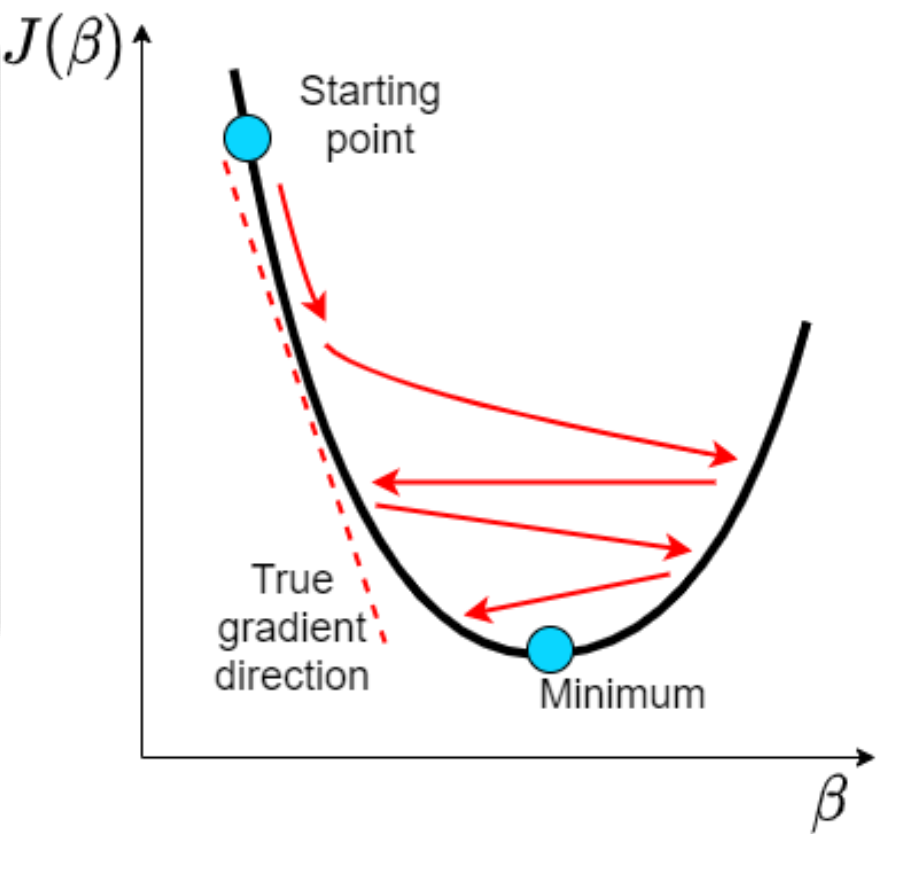
\includegraphics[width=0.5\textwidth]{./figures/chapter_6/graphicsgd.png}
    \caption{Stochastic Gradient Descent}
    \label{fig:stochastic_gradient_descent}
\end{figure}

With respect to the gradient descent:
\begin{itemize}
    \item we are using an instantaneous approximation of the gradient based on individual samples that is \textit{noisy} estimate of the true gradient based on the current sample $d_i$, which means we are not considering the information contained in the other samples and it tells nothing about the average. 
    \item $\beta_i$ is a \textbf{stochastic process}, since it depends on the random samples $d_i$. This adds a source of randomness to the algorithm since $d_i$ changes at each iteration. In fact, if we evaluate $\hat{\nabla J_i}$ for the same $\beta_{i-1}$, we will obtain different values since the function is changed.
    \item Even if not explicitly, we are computing the average \textit{over time} of the gradients of the loss function for each sample.
\end{itemize}

\subsection{Convergence}
Let's call $\beta^\ast$ the exact minimizer of the cost function $J(\beta)$.
\subsubsection*{Constant step-size}
We can show that with constant step-size, the stochastic gradient descent \textit{iterates} (meaning the $\beta_i$) never reach the optimal solution. This is due to the \textit{gradient noise} that is the \textit{inherent} randomness of the gradient. The iterates are \textit{oscillating} around the exact minimizer without reach it effectively.

For a $\mu$ smaller than a certain value (which depends again on $\delta$ and $\nu$), the iterates $\beta_i$ oscillates in a smaller neighbourhood of the true minimizer $\beta^\ast$.

The error $\E{}{\|\beta_i - \beta^\ast\|^2}$ converges to a steady-state error $O(\mu)$ at a geometric rate $O(\rho^i)$ where $\rho \in (0,1)$ is a decreasing function of the step-size $\mu$ and also depends on $\delta$ and $\nu$.

The more smaller is $\mu$ the more are the data that we are averaging, which means that we are considering more the previous information and less the current information. In practice that the stochastic gradient descent with constant step-size allows us to react to data drifts within a fixed number of samples that it is about $\frac{1}{\mu}$. This means that if we set $\mu = 0.01$ we can react to data drifts within 100 samples.

So, the smaller the $\mu$, the smaller will be $\E{}{\|\beta_i - \beta^\ast\|^2}$, but the slower will be the convergence since $\rho$ will increase. 
Summarizing, $\mu$ defines the trade-off between the accuracy of the algorithm and the convergence rate.

\subsubsection*{Decaying step-size}
We can show that with decaying step-size, if $\mu=\mu(i)$ such that $\sum_{i=0}^\infty \mu(i)$ and $\lim_{i\to\infty}\mu(i)=0$ the stochastic gradient descent \textit{iterates} (meaning the $\beta_i$) converge to the exact minimizer and the error $\E{}{\|\beta_i - \beta^\ast\|^2}$ converges to zero.

If $\mu(i) = \frac{\tau}{i+1}$ for $\tau > \frac{1}{\nu}$ the convergence rate it $O(\frac{1}{i})$.

Now, the decaying step-size get more interest because it allows us to reach the minimizer that instead is not reachable with the constant step-size. 


\subsection*{Applications to Online learning}
We can say that decaying step-sizes converge to the exact minimizer but they are not suited to online tasks, because the algorithm cannot react to data drifts since the updates are given less importance due to the increasingly smaller values of $\mu(i)$. We can still use it in \textit{batch} applications rather than online tasks.

By contrast, constant step-sizes are suited to online tasks, but they do not converge to the exact minimizer. However, they converge to a neighbourhood of the minimizer and they are able to react to data drifts. The smaller the $\mu$, the better the accuracy of the algorithm, but the slower the convergence.

\section{Mini-batch Gradient Descent}
The \textbf{mini-batch gradient descent} is a compromise between the gradient descent and the stochastic gradient descent. The idea is to use a \textit{mini-batch} of samples to compute the gradient at each iteration.
\[
    \beta_{i} = \beta_{i-1} - \frac{\mu}{|\mathcal S|}\sum_{i\in \mathcal S} \nabla Q_\beta(d_i)
\]
This variant allows us to reduce the noise within the gradient as we are able to apply the LLN better and obtain more information on the average value of the gradient.

Furthermore, there are versions where you have an \textbf{adaptive step-size} that choose the value of $\mu$ adaptively. Some examples are AdaGrad, Adam, RMSProp.